%!TEX root = ProgCPP_ZF.tex

\part{Vererbung}
\label{sec:Vererbung}

\section{Motivation}
Sie müssen einen Webshop entwickeln. Sie verkaufen Bücher und CDs.\\
Welche Eigenschaften und Methoden benötigen Sie, um ein Buch bzw. eine CD zu charakterisieren?

\section{Artikel als Gemeinsamkeit von Buch und CD}
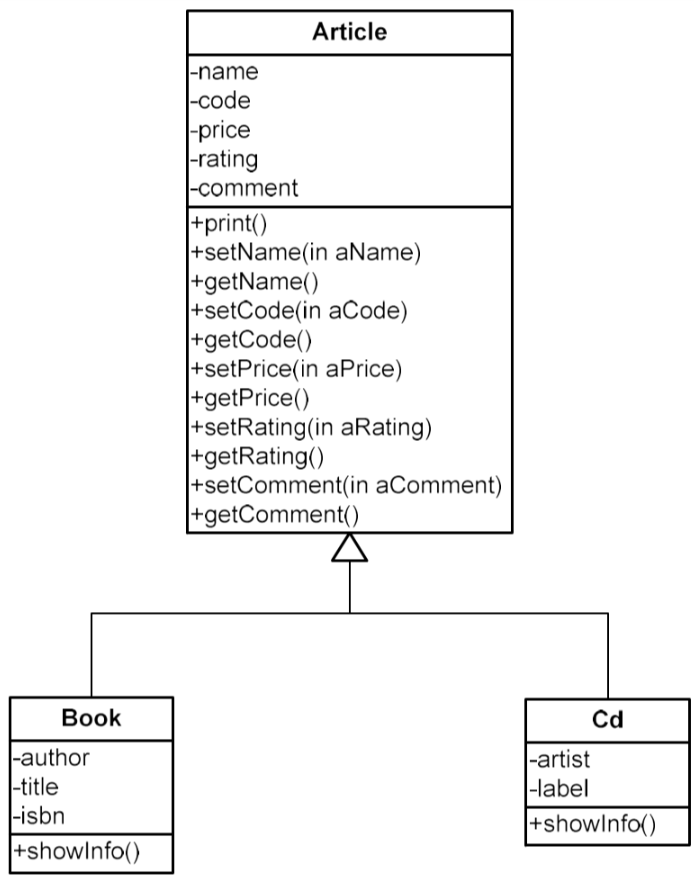
\includegraphics[width=0.3\linewidth]{images/vererbung1.png}

\section{Grundkonzept}
\begin{itemize}
	\item Die Vererbung erlaubt, neue Klassen auf der Basis von bestehenden Klassen zu definieren. Dabei erbt (übernimmt) die neue (Unter-)Klasse alle Eigenschaften der bestehenden (Über-)Klasse.
	\item Man sagt auch, die Oberklasse sei eine Basisklasse, Superclass, Abstraktion oder Generalisierung (Verallgemeinerung).
	\item Die Unterklasse wird auch mit Subclass oder als Spezialisierung bezeichnet.
\end{itemize}

\begin{multicols}{2}
\subsection{Einsatz der Vererbung}
\begin{itemize}
	\item Bestehende Klassen erweitern
	\begin{itemize}
		\item zusätzliche Attribute erweitern
		\item zusätzliche Elementfunktionen
	\end{itemize}
	\item Bestehende Methode einer Basisklasse ändern (überschreiben)
	\item Das Finden von guten Basisklassen ist eine Hauptaufgabe in der Designphase.
\end{itemize}

\subsection{UML-Notation}
\begin{itemize}
	\item Generalisierung/Spezialisierung
	\item \emph{SubClass} erbt sämtliche Eigenschaften von \emph{SuperClass}
	\item ist-ein Beziehung (\emph{SubClass} \textbf{ist eine} \emph{SuperClass})
	\item Pfeilspitze ist ein geschlossenes Dreieck
\end{itemize}
\vfill\null
\columnbreak
\centering{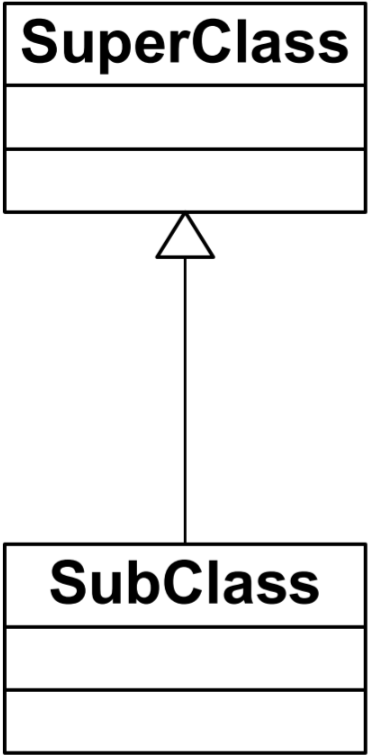
\includegraphics[width=0.3\linewidth]{images/vererbung2.png}}
\end{multicols}

\subsubsection{$"$ist ein$"$-Beziehung}
$"$ist ein$"$-Beziehung ($"$is a$"$-relationship)\\
Beispiel: Baum \textbf{ist eine} Pflanze, Blume \textbf{ist eine} Pflanze.

\subsection{Beispiel: Vererbungshierarchie Lebewesen}
\begin{multicols}{2}
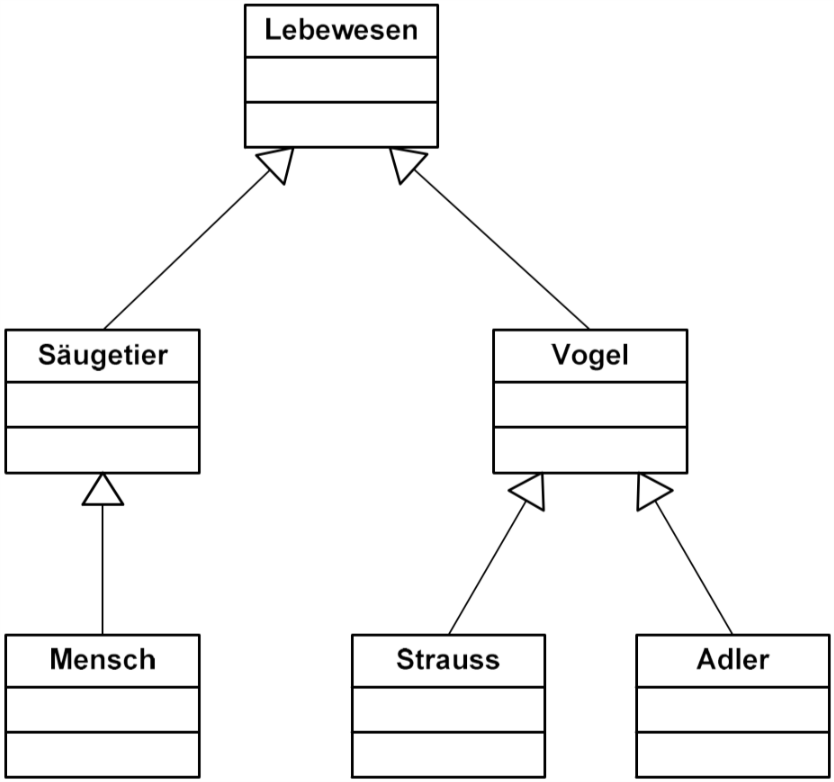
\includegraphics[width=0.7\linewidth]{images/vererbung3.png}
\vfill\null
\columnbreak
\subsubsection{C++-Syntax}
\begin{minipage}{\linewidth}
\vspace{-\baselineskip}
\begin{lstlisting}
class SubClass : public SuperClass
{
	public:
	
	protected:
	
	private:
	
};
\end{lstlisting}
\end{minipage}
\emph{public} ist Normalfall (private und protected sind auch möglich).
\vfill\null
\end{multicols}

\subsubsection{Zugriff auf Elemente der Basisklasse}
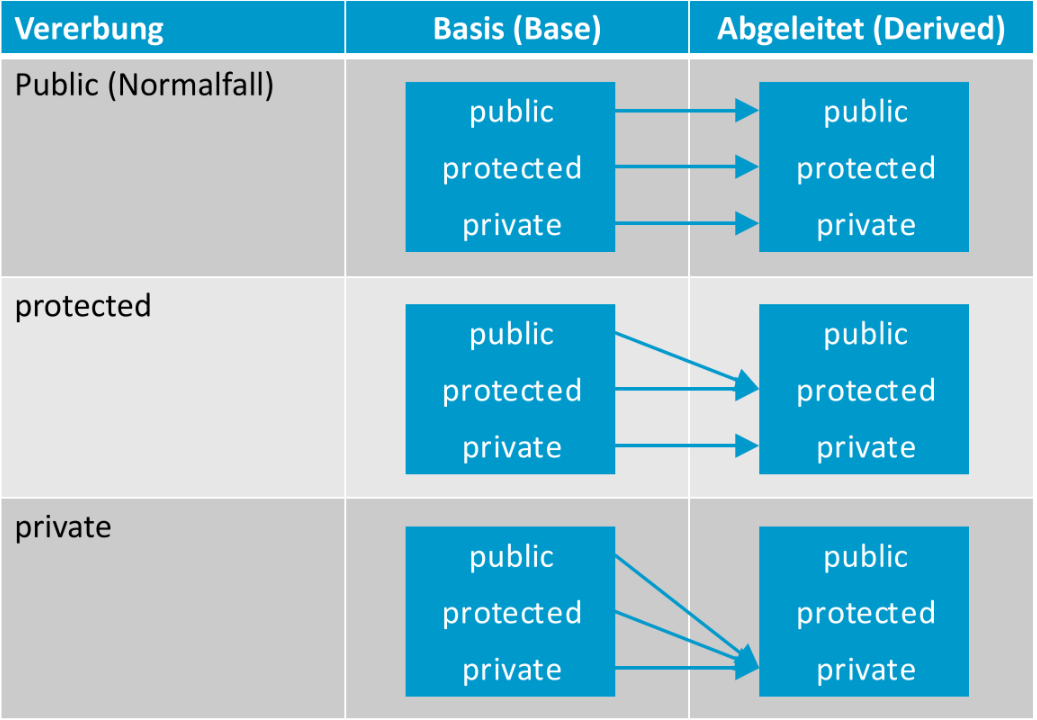
\includegraphics[width=0.5\linewidth]{images/vererbung4.png}

\subsection{Spezifikation von Basisklassen}
\begin{itemize}
	\item Grundsatz: Vererbung sollte immer \emph{public} sein (zu 99,99\%)
	\item Falls bei Vererbung \emph{protected} oder \emph{private} in Betracht gezogen wird, kann der Grund dafür eine falsche Verwendung der Vererbung sein
	\item Für ganz spezifische Anwendungen kann die Vererbung mit \emph{protected} oder \emph{private} sinnvoll sein
\end{itemize}

\subsection{Einsatz von \emph{protected} bei Klassenelementen}
\begin{itemize}
	\item Bei Datenelementen (Attributen) soll \emph{protected} grundsätzlich nicht eingesetzt werden. Attribute sollen generell \emph{private} sein.
	\item Bei Elementfunktionen kann es in Einzelfällen sinnvoll sein, diese als \emph{protected} zu definieren. Dadurch wird der Zugriff gegenüber einer \emph{public}-Sichtbarkeit auf die abgeleiteten Klassen beschränkt.
\end{itemize}
\vfill\null
\pagebreak\newpage

\subsection{Objektgrösse bei der Vererbung}
\begin{itemize}
	\item Ein Objekt einer vererbten Klasse enthält alle Teile der Basisklasse(n) und zusätzlich noch die spezifischen eigenen Teile.
	\item Das Objekt ist somit mindestens so gross wie jenes der Basisklasse(n). (es gibt keine Vererbung $"$by reference$"$)
	\item Wenn Vererbung schlecht eingesetzt wird (z.B. keine is-a-Beziehung), können unnötig grosse Objekte entstehen.
	\item Bei einer Aggregationsbeziehung kann durchaus eine Referenz (oder ein Pointer) auf ein anderes Objekt verwendet werden, d.h. Aggregation $"$by reference$"$ ist möglich.
\end{itemize}

\section{Schlechter (falscher) Einsatz von Vererbung}
Zwischen Wald und Pflanze besteht nicht eine $"$ist-ein$"$ Beziehung. Die richtige Beziehung wäre $"$hat-ein$"$, da ein Wald mehrere Pflanzen hat (folgt später).\\
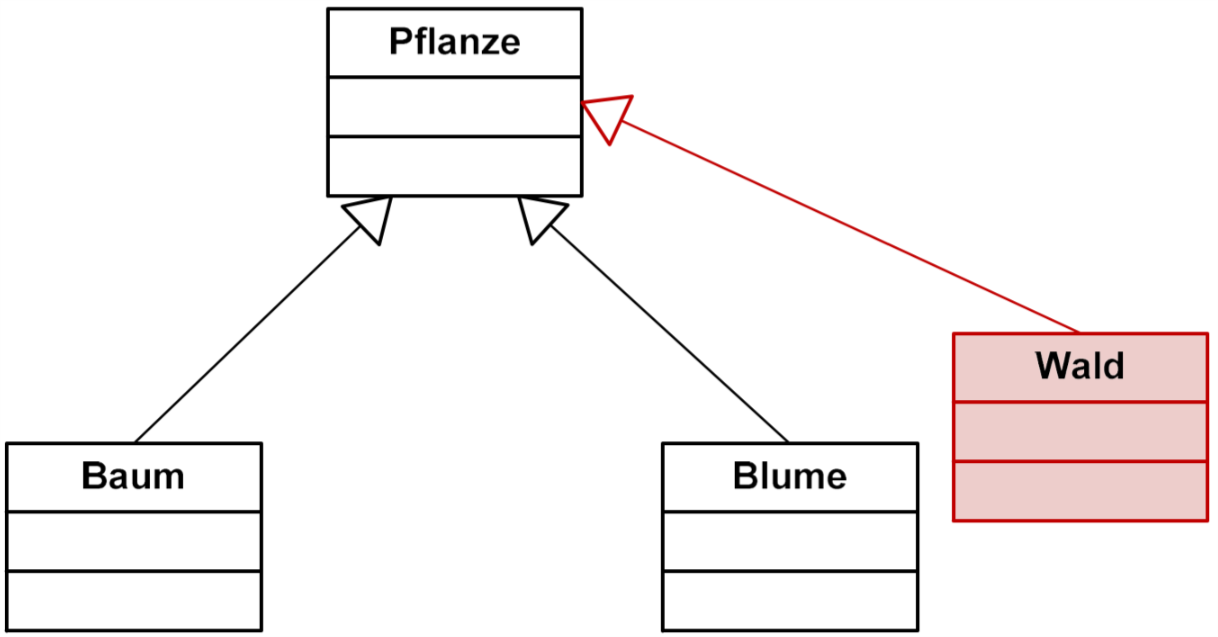
\includegraphics[width=0.5\linewidth]{images/vererbung5.png}

\section{Substitutionsprinzip}
\begin{itemize}
	\item Ein Objekt einer Oberklasse kann Objekte einer beliebigen Unterklasse aufnehmen.
	\item Ein Objekt einer Unterklasse kann keine Objekte der Oberklasse aufnehmen.
	\item[\-]
	\vspace{-\baselineskip}
	\begin{minipage}{0.5\linewidth}
\begin{lstlisting}
class SuperClass{}; 

class SubClass : public SuperClass {};

SuperClass super;
SubClass sub;
super = sub; 	// ok
sub = super;	// geht nicht
\end{lstlisting}
	\end{minipage}
\end{itemize}












